\documentclass[12pt]{article}
\usepackage[utf8]{inputenc}
\usepackage[T1]{fontenc}
\usepackage[english]{babel}
\usepackage[autostyle, english = american]{csquotes}

%%%Margins and Indent 
\setlength{\parindent}{-1pt}
\usepackage{geometry}
\geometry{
 a4paper,
 %total={160mm,250mm},
 left=15mm,
 right = 15mm,
 bottom=15mm ,
 top=15mm,}
 
 %%xcolor
\usepackage{xcolor}
\definecolor{codegreen}{rgb}{0,0.6,0}
\definecolor{codegray}{rgb}{0.5,0.5,0.5}
\definecolor{codepurple}{rgb}{0.58,0,0.82}
\definecolor{backcolour}{rgb}{0.95,0.95,0.92}

 %%%Hyperref
\usepackage{hyperref}
\hypersetup{%
    colorlinks=true,
    citecolor=codegreen, 
    linkcolor=black,
    filecolor=codepurple,      
    urlcolor=codepurple,
}%

%%BibTex
\usepackage[autocite=superscript,backend=biber,style=ieee]{biblatex}
\addbibresource{refs.bib}%Import the bibliography file

%%% Font
%\usepackage{mathptmx}
\usepackage{amsmath,accents}
\usepackage{newtxtext,newtxmath}

%%% images
\usepackage{graphicx}
\usepackage{float}
\usepackage{caption,subcaption}

%%Algorithm
\usepackage[vlined,commentsnumbered]{algorithm2e}
%\usepackage{algpseudocode}

\numberwithin{equation}{section}
\usepackage{tabularx,multirow}

%%Tikz 
\usepackage{tikz}
\usetikzlibrary{angles, quotes, calc, decorations.markings, intersections}
\newcommand{\midlabelline}[3]{
   \node (midlabel) at ($ (#1)!.5!(#2) $) {#3};
   \draw[<-] (#1) --  (midlabel);
   \draw[->] (midlabel) -- (#2);
}

%%import
\usepackage{import}
\usepackage{xifthen}
\usepackage{pdfpages}
\usepackage{transparent}

%%%%defined commands
\newcommand{\pa}{\partial}
\newcommand{\mcm}[1]{\mathcal{#1}}
\newcommand{\bo}{\mcm{O}}
\newcommand{\sDelta}{{\scriptstyle \Delta}}
\newcommand{\gs}{\hspace{0.35cm}}
\newcommand{\mvec}[1]{\accentset{\rightharpoonup}{#1}}
 
%%%%%%
\begin{document}
\baselineskip 0.7cm
\title{\bf \color{black}Computational techniques for solving the Poisson’s equation}
\vskip 3cm
\author{Akarsh Shukla  \\ (2020PHY1216) \and 
Brahmanand Mishra \\ (2020PHY1184) \and 
Shashvat Jain \\ (2020PHY1114) \\[4mm]
{\color{blue}S.G.T.B. Khalsa College, University of
Delhi, Delhi-110007, India.} }

\maketitle
\vskip 4cm
\begin{center}
{\it {\color{blue}Project Report Submitted to}}\\
Dr. Mamta and Dr. H. C. Ramo \\
\textit{\color{blue}as part of internal assessment for the course}\\
 "32223902 - Computational Physics Skills"
\end{center}

\pagenumbering{gobble}

\newpage

\abstract{
    The project report brings light to the application of finite difference method to computationally solve a problem belonging to a class of poisson equation. It covers the extensive analysis of various iterative schemes, namely Jacobi,Gauss-Seidel and SOR, used for solving the system of of linear equations produced by finite difference method.
    This report also includes the conversion of physical problem to a mathematical one by means of normalisation of variables. The iterative schemes have been analysed on the grounds of no. of iterations and  have Results and practices carried out in the making of this report certainly lead the reader to beneficial educational insights into computational physics and its application. \\
    This report is not meant to be a thorough investigation of the problem and should not be seen as a research project.
    }
\newpage
\tableofcontents
\newpage
\pagenumbering{roman}
	\section {Introduction}
    \subsection{Motvation}
    \noindent 
    We first encountered Laplace Equation during our course in electricity and magnetism in second semester and we were fascinated with how one can calculatge the potential in a region just by knowing the boundary condition, ofcourse the region has to be charge free for applying Laplace Equation. After Laplace Equation , we were introduced to Poisson Equation which was able solve in region having charges( or sources ). When we were given the oppurtunity to choose a project in our computational physics charge this semester, it did not take us long to decide the topic for project.
    \subsection{General Idea}
    \noindent
    In our project we will try to tackle the Laplace and Poisson equaton which is an ellipitic linear partial differential equation having application in various fields of physics ranging from thermodynamics, electrostatics etc. We will solve the equation computationally using the method of finite differences in one and two dimensions for rectangular membrane
\section{Theory}
Identical infinitely-long thin metal plates $A_1,A_2,A_3,A_4,A_5,B_1,B_2,B_3 $ and $B_4$ are placed in an \textit{interleaved} arrangement as dipicted in fig1.(a) Group of plates $A_i$ and $B_i$ are connected to the terminal $A$ and $B$ , respectively, by means of gold wires. The terminals are connected to different potential sources $U_A$ and $U_B$ respectively. \\
This is called an interleaved capacitor, Our goal will be to approximate the potential distribution (in two dimensions considering symmetry along the the third axis which will be dropped) inside the capacitor after we disconnect the capacitor from sources, treating the interior plates as line charge distributions.
\begin{align*}
    &U_A = 5V \\
    &U_B = -5V \\
    &\text{Capacitance } = 0.1\mu F\\
    &\text{Distance between plates ($d$)} = 0.5\mu m \\
    &\textit{Dimensions: } 4 \times 4.4 \mu m  
\end{align*}
This arrangement can be seen as a number of parallel plate capacitors connected in parallel to each other as seen in fig1(b),
if $C_0$ is the capacitance of each capacitor in parallel and $C$ is the capacitance of the entire arrangement then,
\begin{align*}
    C_0 = C/8
\end{align*}
Also we know that for parallel plate capacitors with cross-section area $A$ and distance $d$ between the plates,
\begin{align}
    C_0 = \epsilon_0 \frac{A}{d} \implies A = \frac{C_0d}{\epsilon_0}
\end{align}
Therefore the charge distribution on any plate $A_i$ is given by,
\begin{align}
    \rho_A = \frac{(C \times V )}{5A} \implies \rho_A = 2\epsilon_0 \times 10^5C m^{-2} 
\end{align}
Similarly on $B_i$,
\begin{align}
    \rho_B = -2\epsilon_0 \times 10^5C m^{-2} 
\end{align}

\begin{figure}[ht]
    \centering
    \def\svgwidth{0.6\textwidth}
    \import{../diagrams}{capacitor.pdf_tex}
    \caption{Cross-sectional view of interleaved capacitor}
    \label{fig:cap}
\end{figure}

\begin{figure}[ht]
    \centering
    \def\svgwidth{0.6\textwidth}
    \import{../diagrams}{daigram.pdf_tex}
    \caption{Cross-sectional view of the region $\Omega$ in question.}
    \label{fig:}
\end{figure}

Mathematical Formulation:\\
Let $U(x,y)$ and $\vec{E}(x,y)$ be the potential and Electric field distribution defined in the region of our arrangement $(x,y) \in \Omega := [0,4\mu m]\times[0,4.4\mu m]$ .\\
We know from maxwell's laws that for static electric fields $\vec{\nabla} \cdot \vec{E} = \rho / \epsilon_0 $, $\vec{\nabla} \times \vec{E} = 0$
\\
From the later we get $E=-\vec{\nabla}U$, substituting this back into the former we get,
\begin{equation*}
    \vec{\nabla}^2 U = \frac{-\rho}{\epsilon_0}  
\end{equation*}
In two dimensions with euclidean coordinate system the equation reduces to, 
\begin{equation}
    \frac{\pa^2U(x,y) }{\pa x^{2}} + \frac{\pa^2U(x,y) }{\pa y^{2}}= -\frac{\rho(x,y)}{\epsilon_0} \\
\end{equation}
where,
\begin{equation}
\rho(x,y) =  \begin{cases}
    -2\epsilon_0 \times 10^5 C m^{-2} & :\text{if} \gs (x,y) \in B_i \gs \text{where} \gs i = 1,2,3,4 \\
    2\epsilon_0 \times 10^5 C m^{-2} & :\text{if} \gs (x,y) \in A_i \gs \text{where} \gs i = 2,3,4  \\
    0 C m^{-2} & : \gs \text{elsewhere}
\end{cases}  
\end{equation}
Now according to our given arrangement,
\begin{align}
    B_1 &= \{ (x^*,y^*) \gs : \gs x^*= 0.5\mu m \gs;\gs 0.4\mu m \leq y^* \leq 4.4\mu m \} \\
    B_2 &= \{ (x^*,y^*) \gs : \gs x^*= 1.5\mu m \gs;\gs 0.4\mu m \leq y^* \leq 4.4\mu m \} \\
    B_3 &= \{ (x^*,y^*) \gs : \gs x^*= 2.5\mu m \gs;\gs 0.4\mu m \leq y^* \leq 4.4\mu m \} \\
    B_4 &= \{ (x^*,y^*) \gs : \gs x^*= 3.5\mu m \gs;\gs 0.4\mu m \leq y^* \leq 4.4\mu m \} \\
    A_2 &= \{ (x^*,y^*) \gs : \gs x^*= 1\mu m \gs;\gs 0\mu m \leq y^* \leq 4\mu m \} \\
    A_3 &= \{ (x^*,y^*) \gs : \gs x^*= 2\mu m \gs;\gs 0\mu m \leq y^* \leq 4\mu m \} \\
    A_4 &= \{ (x^*,y^*) \gs : \gs x^*= 3\mu m \gs;\gs 0\mu m \leq y^* \leq 4\mu m \} 
\end{align}
We get the following boundary conditions for the above boundary value problem,
\begin{align}
    & U(0,y) = +5 V \gs; \gs U(4,y) = +5 V \\ 
    & U_y(x,0) = 0V/m \gs; \gs U_y(x,4.4) = 0V/m 
\end{align}

Non-Dimensionalizing the variables, \autocite{tudortmundkuzmin2}

Let new dimensionless variables,
\begin{align}
    x' = \frac{x}{s} \gs \gs y' = \frac{y}{s} \gs \gs U' = \frac{U}{\nu}
\end{align}
where $s$ and $\nu$ are known constant scaling factors having dimensions of length and electric potential respectively.

The B.V.P reduces to,
\begin{equation}
    \frac{\pa^2U'(x',y') }{\pa x^{'2}} + \frac{\pa^2U'(x',y') }{\pa y^{'2}}= -\frac{\rho'(x',y') s^2}{\epsilon_0 \nu} \\
\end{equation}
where,
\begin{equation}
\rho'(x',y') =  \begin{cases}
    -2\epsilon_0 \times 10^5  & :\text{if} \gs (x',y') \in B_i \gs \text{where} \gs i = 1,2,3,4 \\
    2\epsilon_0 \times 10^5 & :\text{if} \gs (x',y') \in A_i \gs \text{where} \gs i = 2,3,4 \\
    0  & : \gs \text{elsewhere}
\end{cases}
\end{equation}
Now according to our given arrangement,
\begin{align}
    B_1 &= \{ (x^*,y^*) \gs : \gs x^*= 0.5/s \gs;\gs 0.4/s \leq y^* \leq 4.4/s \} \\
    B_2 &= \{ (x^*,y^*) \gs : \gs x^*= 1.5/s \gs;\gs 0.4/s \leq y^* \leq 4.4/s \} \\
    B_3 &= \{ (x^*,y^*) \gs : \gs x^*= 2.5/s \gs;\gs 0.4/s \leq y^* \leq 4.4/s \} \\
    B_4 &= \{ (x^*,y^*) \gs : \gs x^*= 3.5/s \gs;\gs 0.4/s \leq y^* \leq 4.4/s \} \\
    A_2 &= \{ (x^*,y^*) \gs : \gs x^*= 1/s \gs;\gs 0/s \leq y^* \leq 4/s \} \\
    A_3 &= \{ (x^*,y^*) \gs : \gs x^*= 2/s \gs;\gs 0/s \leq y^* \leq 4/s \} \\
    A_4 &= \{ (x^*,y^*) \gs : \gs x^*= 3/s \gs;\gs 0/s \leq y^* \leq 4/s \} 
\end{align}
We get the following boundary conditions for the above boundary value problem,
\begin{align}
    & U(0,y) = +5/\nu \gs; \gs U(4,y) = +5/\nu \\ 
    & U_y(x,0) = 0 \gs; \gs U_y(x,4.4) = 0 
\end{align}

%%%%%%%%%%%%%%%END%%%%%%%%%%%%%%%%%%%%%%
\section{Methodology}
\subsection{Finite Difference Method}
Finite Difference Methods(FDM) are used for approximating the solution of partial differential equations over a set of finite points, arranged in a geometrical structure called a \textbf{mesh}%
\footnote[1]{An object which consists of points which are spaced in a specific geometrical pattern is referred to as a \textbf{mesh} and each point in this mesh is called a \textbf{node}. The distance between any two adjacent nodes in a mesh with uniform spacing is called its \textbf{meshsize}}%
, in the continous domain of solution. The methods involve the idea of reducing the given PDE, by means of truncated taylor series approximation of the derivatives, to a difference equation which is much easier to digest numerically. 
\subsubsection{Finite Difference Approximations}
The quality of the solution depends on the quality of approximations made to the derivatives.
%%%
Consider this one-dimensional structured mesh of nodes $(x_0,x_1,x_2,..,x_i,..,x_n)$ at which the solution $U(x_i)$  is to be found, such that the difference $h = x_{i+1} - x_i $ is constant throughout the mesh and $x_i \equiv x_0 + ih$.\\
\begin{figure}[h]
\centering

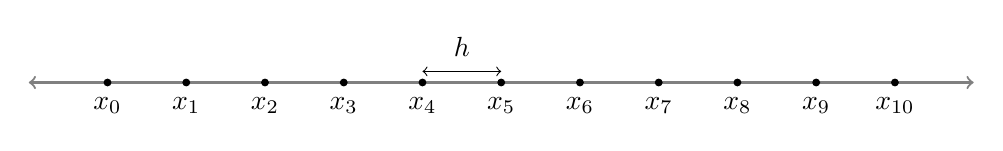
\begin{tikzpicture}
    \coordinate (H) at (4.5,6pt);
    \draw[thick,color=gray,<->] (-1,0) -- (11,0);
    \foreach \x  in {0,1,2,3,4,5,6,7,8,9,10}
        \draw[fill=black] (\x cm,0) circle (1.2pt) (\x cm,-2pt) node[anchor=north] {$x_{\x}$};
    \draw[thin,<->] (4,4pt) -- (5,4pt);%
    \node[anchor=south] at (H) {$h$};
\end{tikzpicture}

\caption{\small 1D mesh with 11 nodes and a meshsize h}
\end{figure}
\\
Let $U_i$ represent the solution at the $i$-th node and \hfill
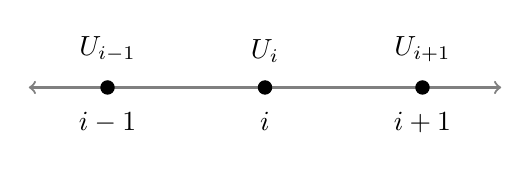
\begin{tikzpicture}[scale =2]
    \draw[thick,color=gray,<->] (3,-2cm) -- (6,-2cm);
    \foreach \x  in {3.5,4.5,5.5}
        \draw[fill=black] (\x cm,-2cm) circle (1.2pt) ;
    \draw (3.5 cm,-2.01cm) node[anchor=north,shift={(0,-5pt)}] {$i-1$};
    \draw (4.5 cm,-2.01cm) node[anchor=north,shift={(0,-5pt)}] {$i$};
    \draw (5.5 cm,-2.01cm) node[anchor=north,shift={(0,-5pt)}] {$i+1$};
    \draw (3.5 cm,-1.99cm) node[anchor=south,shift={(0,5pt)}] {$U_{i-1}$};
    \draw (4.5 cm,-1.99cm) node[anchor=south,shift={(0,5pt)}] {$U_{i}$};
    \draw (5.5 cm,-1.99cm) node[anchor=south,shift={(0,5pt)}] {$U_{i+1}$};
\end{tikzpicture}
\begin{equation*}
    \left. \frac{\partial U}{\partial x} \right|_{x_ i} = U_{x}(x_0 + ih) \equiv U_{x}|_i
\end{equation*} 
\begin{equation*}
    \left. \frac{\partial^2 U}{\partial x^2} \right|_{x_ i} = U_{xx}(x_0 + ih) \equiv U_{xx}|_i
\end{equation*}

The first order derivative can be defined as,
{\raggedright 
\begin{align*}
    &\text{} \hspace{1cm} U_x|_i = \lim_{h \to 0} \frac{U_{i+1} - U_i}{h}  \\
    &\text{or,} \hspace{1cm} U_x|_i = \lim_{h \to 0} \frac{U_{i} - U_{i-1}}{h}  \\
    &\text{or,} \hspace{1cm} U_x|_i = \lim_{h \to 0} \frac{U_{i+1} - U_{i-1}}{2h}  
\end{align*}
}

Finite difference approximations are obtained by dropping the limit and can be written as, 
 
\begin{flalign*}
    &\text{Forward Difference} \hspace{1cm} U_x|_i \approx \frac{U_{i+1} - U_i}{h} \equiv \delta^+_{x} U_i  \\
    &\text{Backward Difference} \hspace{1cm} U_x|_i \approx \frac{U_{i} - U_{i-1}}{h} \equiv \delta^-_{x} U_i \\
    &\text{Central Difference} \hspace{1cm} U_x|_i \approx \frac{U_{i+1} - U_{i-1}}{2h} \equiv \delta_{2x} U_i 
\end{flalign*}

Where $\delta^+_{x} , \delta^-_{x} , \delta_{2x}$ are called the \textbf{finite diference operators} for approximating \textbf{first-order derivatives} and their expansion is called the \textbf{finite difference quotient}, each representing forward,backward and centered respectively.
Second and Higher order finite difference Quotients can also be obtained,
\begin{align*}
    U_{xx}|_i &= \lim_{h \to 0} \frac{U_x(x_i+\frac{h}{2}) - U_x(x_i-\frac{h}{2})}{h} \\
    &= \lim_{h \to 0} \frac{1}{h} \left[{\frac{U(x+h) - U(x)}{h} - \frac{(U(x)- U(x-h))}{h}}\right]\\
    &= \lim_{h \to 0}\frac{U_{i+1}-2 U_i + U_{i-1}}{h^2} \\
    &\approx \boxed{\delta^2_x U_i \equiv \frac{1}{h^2}(U_{i+1}-2 U_i + U_{i-1})} \hspace{1cm} \text{[Central second-order Difference]}
\end{align*}

\begin{figure}[ht]
    \centering
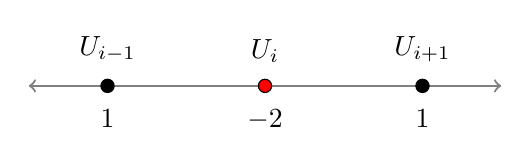
\begin{tikzpicture}[scale=2]
    \coordinate (A) at (3.5 cm,0cm);
    \coordinate (B) at (4.5 cm,0cm);
    \coordinate (C) at (5.5 cm,0cm);
    \draw[thick,color=gray,<->] (3cm,0) -- (6cm,0);
    \draw[fill=black] (A) circle (1.2pt) (A) node[anchor=north,shift={(0,-5pt)}] {$1$};
    \draw[fill=red] (B) circle (1.2pt) (B) node[anchor=north,shift={(0,-5pt)}] {$-2$};
    \draw[fill=black] (C) circle (1.2pt) (C) node[anchor=north,shift={(0,-5pt)}] {$1$};
    \draw (A) node[color=black,anchor=south,shift={(0,5pt)}] {$U_{i-1}$};
    \draw (B) node[color=black,anchor=south,shift={(0,5pt)}] {$U_{i}$};
    \draw (C) node[color=black,anchor=south,shift={(0,5pt)}] {$U_{i+1}$};
\end{tikzpicture}
\end{figure}

The vector of coefficients of the function values at various nodes forms what is called the \textbf{stencil} of the finite difference operator and it uniquely idetifies the operator. The combination $(1,-2,1)$ is called a \textbf{three point stencil} as it combines function values from three different points on the mesh.
It is fairly obvious to notice that any finite difference operator for any derivative at any node is just a linear combination of the function values at various neighbourhood nodes.   

\subsubsection{Local Truncation Error of Finite Difference Approximations}
The \textit{'error'} that accompanies \textit{'approximations'} in the method must be acccounted for. In this section, the truncation error in the derivative approximations is ascertained which will later help us deduce the error in PDE's solved using these approximations.
\\[2mm]
\textbf{The local truncation error for derivative approximations} is defined here as the difference between the exact value of the derivate and the approximated value at node $i$, it can be calculated using Taylor series expansions about $i$,\\[2mm]
For Forward difference operator,\autocite{mitocw}\autocite{thomas2013numerical}
\begin{align*}
    \tau &\equiv \delta _ x^{+} U_ i - {U_ x}|_ i \\
    &= \frac{1}{\sDelta x}\left( U_ {i+1} - U_{i}\right) - {U_ x}|_i \\
    &= \frac{1}{\sDelta x}\left[ \left( U_ i + \sDelta x{U_ x}|_ i + \frac{1}{2}(\sDelta x)^2{U_{xx}}|_ i + \mcm{O}((\sDelta x)^3)\right) - U_i \right] - {U_ x}|_ i \\
    &= \frac{1}{2}\sDelta x{U_{xx}}|_ i + \mcm{O}((\sDelta x)^2) = \mcm{O}(\Delta x)
\end{align*}
For Backward difference operator, 
\begin{align*}
    \tau &\equiv \delta _ x^{-} U_ i - {U_ x}|_ i \\
    &= \frac{1}{\sDelta x}\left( U_ i - U_{i-1}\right) - {U_ x}|_i \\
    &= \frac{1}{\sDelta x}\left[ U_ i - \left( U_ i - \sDelta x{U_ x}|_ i + \frac{1}{2}(\sDelta x)^2{U_{xx}}|_ i + \mcm{O}((\sDelta x)^3)\right)\right] - {U_ x}|_ i \\
    &= -\frac{1}{2}\sDelta x{U_{xx}}|_ i + \mcm{O}((\sDelta x)^2) = \mcm{O}(\Delta x)  
\end{align*}
For Central difference operator,
\begin{align*}
    \tau &\equiv \delta _ {2x} U_ i - {U_ x}|_ i \\
    &= \frac{1}{{2 \sDelta } x}\left( U_ {i+1} - U_{i-1}\right) - {U_ x}|_i \\
    &= \frac{1}{2 \sDelta  x}\Bigg[ \left( U_ i + \sDelta x{U_ x}|_ i + \frac{1}{2}(\sDelta x)^2{U_{xx}}|_ i + \frac{1}{6}(\sDelta x)^3{U_{xxx}}|_ i + \frac{1}{12}(\sDelta x)^4{U_{xxxx}}|_ i + \mcm{O}((\sDelta x)^5)\right) \\
    &\qquad - \left( U_ i - \sDelta x{U_ x}|_ i + \frac{1}{2}(\sDelta x)^2{U_{xx}}|_ i - \frac{1}{6}(\sDelta x)^3{U_{xxx}}|_ i + \frac{1}{12}(\sDelta x)^4{U_{xxxx}}|_ i +\mcm{O}((\sDelta x)^5)\right)\Bigg] - {U_ x}|_ i \\
    &= -\frac{1}{6}\Delta x^2 U_{xxx_ i} + \mcm{O}((\sDelta x)^4) = \mcm{O}((\Delta x)^2)
\end{align*}
where in the above expressions we assume that the Higher order derivatives of $U$ at $i$ are well defined. For a fairly small $\Delta x$ (less than 1) we can confidently say that $\bo(\Delta x^2)$ is samller than $\bo(\Delta x)$%
\footnote{The definition of the "big $\bo$" notation says that if for given functions $f(x)$ and $g(x)$ for $x \in S$ where S is some subset of $\mathbf{R}$, there exists a positive constant A such that $|f(x)| \leq A|g(x)|$ $\forall$ $x \in S$, we say that $f(x)$ is the "big $\bo$" of $g(x)$ or that $f(x)$ is of order of $g(x)$, mathematically given by $f(x) = \bo(g(x))$}%
. Thus we note that the centered difference approximation (second-order accurate) approximates the derivative more accurately than either of the \textit{one-sided diferences} which are first-order accurate.\footnote{Forward and Backward differences are also called one-sided differences}

Similarly, Approximation of second-order derivative,
\begin{align*}
    \tau &\equiv \delta^2_x U_i - U_{xx}|_i \\
     &= \frac{1}{(\sDelta x)^2}(U_{i+1}-2 U_i + U_{i-1})  - U_{xx}|_i \\
     &= \frac{1}{(\sDelta x)^2}\Bigg[ \left( U_ i + \sDelta x{U_ x}|_ i + \frac{1}{2}(\sDelta x)^2{U_{xx}}|_ i + \frac{1}{6}(\sDelta x)^3{U_{xxx}}|_ i + \frac{1}{12}(\sDelta x)^4{U_{xxxx}}|_ i + \mcm{O}((\sDelta x)^5)\right) - 2 U_i\\
    & + \left( U_ i - \sDelta x{U_ x}|_ i + \frac{1}{2}(\sDelta x)^2{U_{xx}}|_ i - \frac{1}{6}(\sDelta x)^3{U_{xxx}}|_ i + \frac{1}{12}(\sDelta x)^4{U_{xxxx}}|_ i +\mcm{O}((\sDelta x)^5)\right)\Bigg] - {U_ {xx}}|_ i \\
    &= \mcm{O}((\sDelta x)^2)
\end{align*}
Thus, the second-order derivative approximator is also second order accurate.

%%Second derivate %%
\subsubsection{Reducing PDE to a discretised difference equation}
First we decompose our continous domain $\Omega$ of $U(x,y)$ to a discretised one by overlaying it with a uniformly structured rectangular mesh of meshsize $\sDelta x=\sDelta y= h$ and working only on the nodes of the mesh. \\[2mm]

\begin{figure}
    \centering
    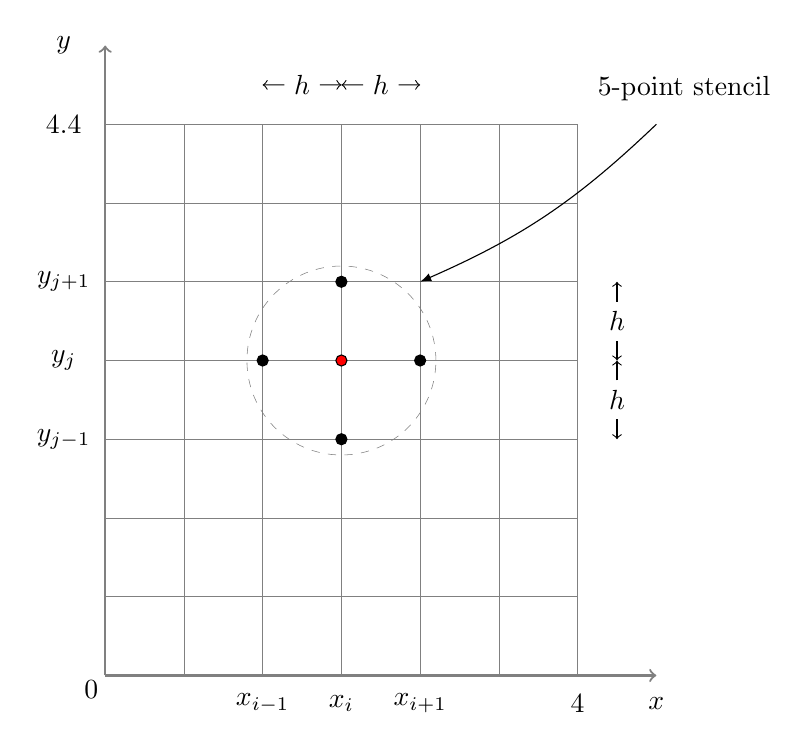
\begin{tikzpicture}
    \coordinate (Y) at (-15pt,8);
    \coordinate (X) at (7,-10pt);
    \draw[step = 1cm,gray, very thin] (0,0) grid (6,7);
    \draw[thick,color=gray,->] (0,0) -- (7,0);
    \draw[thick,color=gray,->] (0,0) -- (0,8);
    \draw (X) node {$x$};
    \draw (Y) node {$y$};
    \draw (X) node[shift={(-4,0)}] {$x_i$};
    \draw (Y) node[shift={(0,-4)}] {$y_j$};
    \draw (X) node[shift={(-5,0)}] {$x_{i-1}$};
    \draw (Y) node[shift={(0,-5)}] {$y_{j-1}$};
    \draw (X) node[shift={(-3,0)}] {$x_{i+1}$};
    \draw (Y) node[shift={(0,-3)}] {$y_{j+1}$};
    \draw (Y) node[shift={(0,-1)}] {$4.4$};
    \draw (X) node[shift={(-1,0)}] {$4$};
    \midlabelline{[shift={(-0.5,3cm + 10pt)}]X}{[shift={(-0.5,4cm +10pt)}]X}{$h$};
    \midlabelline{[shift={(-0.5,4cm +10pt)}]X}{[shift={(-0.5,5cm +10pt)}]X}{$h$};
    \coordinate (Xa) at ([shift={(2cm +15pt,-0.5)}]Y); 
    \coordinate (Xb) at ([shift={(3cm +15pt,-0.5)}]Y); 
    \coordinate (Xc) at ([shift={(4cm +15pt,-0.5)}]Y); 
    \midlabelline{Xa}{Xb}{$h$};
    \midlabelline{Xb}{Xc}{$h$};
    \draw (0,0) node[shift={(-5pt,-5pt)}] {$0$};
    \draw[fill=red] (3,4) circle (2pt) ;
    \draw[fill=black] (4,4) circle (2pt) ;
    \draw[fill=black] (2,4) circle (2pt) ;
    \draw[fill=black] (3,3) circle (2pt) ;
    \draw[fill=black] (3,5) circle (2pt) ;
    \draw[dashed,very thin,color=gray] (3,4) circle (1.2cm) ;
    \draw [latex-] (4cm,5cm) to [bend right=10] (7,7) node[anchor=south,shift={(10pt,5pt)}] {$5$-point stencil};
\end{tikzpicture}
\end{figure}
\noindent
Therefore we have,$U_{i,j} = U(x_i,y_j)$ and $\rho_{i,j} = \rho(x_i,y_j)$ $\forall \gs i \in \{0,1,\dots,N_x\} ; \gs j \in \{0,1,\dots,N_y\} $. \\[2mm] where $N_x = \frac{4}{h} $ and  $N_y = \frac{4.4}{h}$ \\[2mm]   
We replace the second-order derivatives in partial differential equation (2.16) with central difference operators,
\begin{align}
    &\delta^2_x U_{i,j} + \delta^2_y U_{i,j} = - \frac{\rho'_{i,j} s^2}{\epsilon_0 \nu} \\
    &\frac{1}{h^2}(U_{i+1,j}+ U_{i-1,j} -4 U_{i,j} + U_{i,j+1}+ U_{i,j-1}) = - \frac{\rho'_{i,j} s^2}{\epsilon_0 \nu}
\end{align}

After rearranging we obtain the useful relation,
\begin{align} \label{eq:difference equation}
    U_{i,j} = \frac{1}{4} \left[ U_{i+1,j}+ U_{i-1,j} + U_{i,j+1}+ U_{i,j-1} + h^2\frac{\rho'_{i,j} s^2}{\epsilon_0 \nu} \right] \\ \gs \forall \gs i \in \{1,2,\dots,N_x-1\} ; \gs j \in \{0,1,\dots,N_y\} 
\end{align}

The Dirichlet boundary conditions get translated to,
\begin{align*}
    U_{i,j} = 5 \gs \forall \gs i \in \{0,N_x\} ; \gs j \in \{0,1,\dots,N_y\}
\end{align*}
and Neumann to,
\begin{align*}
    &U_{i,j+1} = U_{i,j-1} \gs \forall \gs j = N_y ; \gs i \in \{0,1,\dots,N_x\} \\
    &U_{i,j-1} = U_{i,j+1} \gs \forall \gs j = 0 ; \gs i \in \{0,1,\dots,N_x\} 
\end{align*}
\subsection{Iterative methods to solve linear algebraic equations}

In the last section we have discussed how to reduce a PDE to a linear combination of function values at various nodes by means of the method of finite differences. If we let the function value at any node as an unknown variable then the stencil when applied to all interior nodes gives rise to a system of linear algebraic equations, which may be very large. A two-dimensional problem like ours may lead to a system of several thousand unknowns, and three-dimensional problems involving several hundred thousand unknowns are common in real engineering situations. The solution of such a system is a major problem in itself as traditional methods like Gaussian-elimination result in large computation times, we are therefore forced to employ faster methods. As we have seen above, the system of equations produced by a discretisation has many special features and an efficient solution procedure must exploit these. The most obvious property of the system is that it is extremely sparse. Even when there are many thousand unknowns, each equation will involve one unknown and the unknowns at its immediate neighbourhood. In particular, if we write the equations in the conventional notation,
\begin{equation} \label{linear system}
    A \mvec{x} = \mvec{b} 
\end{equation}
where A is an N × N matrix, b the given data vector and x the vector of N unknown interior mesh values, there is an implied one-dimensional ordering of these values which is somewhat unnatural and obscures the important property that only immediate neighbours are involved. Each row of the matrix A involves only a very small number of non-zero elements, commonly five or seven; moreover in many problems a suitable ordering of the unknowns will lead to a matrix in which these non-zero elements occur in a regular pattern. Instead of solving for this vector equation in matrix form we solve by applying the Finite difference equation to each node in the mesh which in practice is the same as solving the vector equation \ref{linear system} but without explicitly stating the matrices $A$ and $b$. Following sections describe the various methods we successfully employed for the same.\autocite{mortonpde}\autocite{tudortmundkuzmin}
\subsubsection{Jacobi Method}
Jacobi method starts with a set of intial guess values for the unknowns and then gets new value for the unkowns by substituting the quess values in the equations one at a time,the process is repeated with the newly produced value of the unkowns.\\[2mm]
\begin{algorithm}[H]
    \textbf{Jacobi Method (X,P,h,$\mathbf{\epsilon_r}$)}\\[-1pt]  
    This verison of jacobi method is optimised for poisson on a uniformly structured rectangular mesh, It takes the initial guess values at all nodes, the stencil and iteratively solves the stencil over all interior nodes unitl the relative tolerance is reached.  \\[2mm]
	\KwIn{ $\mathbf{X^{(0)}} :\gs N_x \times N_y $ matrix of initial guess values, value of step size $h$, a matrix containing the initial charge configuration $\mathbf{P}$, N an upper bound on the number of iterations} 
	\KwOut{$\mathbf{X^{(n*)}} $ matrix containing the values of potential on all satisfying the relation \ref{eq:difference equation}} 
    \For{n in $1,\dots N$}{ 
		\For{i = $1,2,3,\cdots,N_x-1$}{
            \For{j = $0,1,2,\cdots,N_y$}{
                \If{j = 0 }{
                    $X^{(n)}_{i,j-1} = X^{(n)}_{i,j+1}$
                }
                \If{j = $N_y$ }{
                    $X^{(n)}_{i,j+1} = X^{(n)}_{i,j-1}$
                }
            $X^{(n+1)}_{i,j} = \frac{1}{4} \left[ X^{(n)}_{i+1,j}+ X^{(n)}_{i-1,j} + X^{(n)}_{i,j+1}+ X^{(n)}_{i,j-1} + h^2\frac{P_{i,j} s^2}{\epsilon_0 \nu} \right]$
        }}
        \If{$\max_{i,j}{\{\frac{X^{(n+1)} -X^{{(n)}}}{X^{(n+1)}}\}}\leq \epsilon_r$}{
            return Output \\
            break
        }
    }
    \caption{Jacobi Method}
\end{algorithm}


\subsubsection{Gauss-Seidel Method}
The Gauss-Seidel method applies the stencil on the new unkowns as it iterates over the system of equations unlike Jacobi method which only works on the unknown values of the previous iteration.\\[2mm]
\begin{algorithm}[H]
    \textbf{Gauss-Seidel Method (X,P,h,$\mathbf{\epsilon_r}$)}\\[-1pt]
    This verison of jacobi method is optimised for poisson on a uniformly structured rectangular mesh, It takes the initial guess values at all nodes, the stencil and iteratively solves the stencil over all interior nodes unitl the relative tolerance is reached.  \\[2mm]
	\KwIn{ $\mathbf{X^{(0)}} :\gs N_x \times N_y $ matrix of initial guess values, value of step size $h$, a matrix containing the initial charge configuration $\mathbf{P}$, N an upper bound on the number of iterations} 
	\KwOut{$\mathbf{X^{(n*)}} $ matrix containing the values of potential on all satisfying the relation \ref{eq:difference equation}} 
    \For{n in $1,\dots N$}{ 
		\For{i = $1,2,3,\cdots,N_x-1$}{
            \For{j = $0,1,2,\cdots,N_y$}{
                \If{j = 0 }{
                    $X^{(n+1)}_{i,j-1} = X^{(n)}_{i,j+1}$
                }
                \If{j = $N_y$ }{
                    $X^{(n)}_{i,j+1} = X^{(n)}_{i,j-1}$
                }
            $X^{(n+1)}_{i,j} = \frac{1}{4} \left[ X^{(n)}_{i+1,j}+ X^{(n+1)}_{i-1,j} + X^{(n)}_{i,j+1}+ X^{(n+1)}_{i,j-1} + h^2\frac{P_{i,j} s^2}{\epsilon_0 \nu} \right]$
        }}
        \If{$\max_{i,j}{\{\frac{X^{(n+1)} -X^{{(n)}}}{X^{(n+1)}}\}}\leq \epsilon_r$}{
            return Output \\
            break
        }
    } 
    \caption{Jacobi Method}
\end{algorithm}


\subsubsection{Successive Over-Relaxation(SOR)}
Successive over-relaxation or SOR is a method that belongs to a class of methods called Relaxation methods. 
Such so-called relaxation methods reached a high state of development in the l940s One result was a modification of the Gauss–Seidel procedure which is now called successive over-relaxation or the SOR method.
Taking the recent values of the unknowns. We proceed by calculating the correction which would be given by the Gauss–Seidel iteration (iterating on new unknowns), and then multiply this correction by $\omega$ before adding to the previous value. The term over-relaxation then implies that $\omega>1$. \\[2mm]

\begin{algorithm}[H]
    \textbf{S.O.R Method (X,P,h,$\mathbf{\epsilon_r},\omega$)}\\[-1pt]
    This verison of jacobi method is optimised for poisson on a uniformly structured rectangular mesh, It takes the initial guess values at all nodes, the stencil and iteratively solves the stencil over all interior nodes unitl the relative tolerance is reached.  \\[2mm]
	\KwIn{ $\mathbf{X^{(0)}} :\gs N_x \times N_y $ matrix of initial guess values, value of step size $h$, a matrix containing the initial charge configuration $\mathbf{P}$, N an upper bound on the number of iterations,$\omega$ the relaxation factor} 
	\KwOut{$\mathbf{X^{(n*)}} $ matrix containing the values of potential on all satisfying the relation \ref{eq:difference equation}} 
    \For{n in $1,\dots N$}{ 
		\For{i = $1,2,3,\cdots,N_x-1$}{
            \For{j = $0,1,2,\cdots,N_y$}{
                \If{j = 0 }{
                    $X^{(n+1)}_{i,j-1} = X^{(n)}_{i,j+1}$
                }
                \If{j = $N_y$ }{
                    $X^{(n)}_{i,j+1} = X^{(n)}_{i,j-1}$
                }
            $X^{(n+1)}_{i,j} = X^{(n)}_{i,j} + \omega\left(\frac{1}{4} \left[ X^{(n)}_{i+1,j}+ X^{(n+1)}_{i-1,j} + X^{(n)}_{i,j+1}+ X^{(n+1)}_{i,j-1} + h^2\frac{P_{i,j} s^2}{\epsilon_0 \nu} \right]-X^{(n)}_{i,j}\right)$
        }}
        \If{$\max_{i,j}{\{\frac{X^{(n+1)} -X^{{(n)}}}{X^{(n+1)}}\}}\leq \epsilon_r$}{
            return Output \\
            break
        }
    } 
    \caption{SOR Method}
\end{algorithm}                                    


\section{Numerical Analysis}
In this section we will try to analyse  results thoroughly. In this section we will analyse the Jacobi Method, SOR  and Gauss Seidel Method  
\subsection{Main Problem}
our problem consists of 4 capacitor which were charged at the beginning and then disconnnected after they were charged  to a potential of $ \pm5 volts$. So in our problem the first plate of capacitor at the begining {(i.e. $A_{1}$ in figure 1) }of system and last plate {(i.e. $A_5$)} of the last capacitor  would act as the boundary condition. We are solving our problem by considering it only in two direction and not taking the third direction due to the symmetry of problem.
\subsubsection{Expectation}
Now since in our problem there are 4 capacitor and all of them have identical condition in the begining so we expect to get symmetrical result with high potential near the positively chacged plates (i.e. the plates denoted by A  in the figure1) of capacitor and low potential near the negatively charged plates but we are considerig them in two dimension so they will behave as the "line charges " rather than the capacitors.Since we are ensuring the value at the boundary reamins constant at $ +5 volts $ so the distribution should contain the positive spike in value of potential at the location of " line charges " having positive potential at the begining and negative spike at places of negative potential. \\
Now if we anlayse the our set up from ones side then, at the top of arrangement we have boundary in form of line charge whose potential is 5 volts and then we line charge $ B_1$ which was charged to a potential of $ -5 volts $ so we should expect a decrease in potential as we move from $ A_1 $ to $ B_1 $ in x direction with spike at $ B_1 $ and since the potential is not maintained in Y direction so we should expect a decrease in potential from one side of Y to other, now after $ B_1 $ we move to $ A_2 $ so we should expect increase in potential with positive spike at $ A_2 $ in x direction and since the $ A_2 $ line charge extend till only $ 4 \mu m $ and its predecessor and successor which are both negatively charged exist for $ 4.4 \mu m $ so we should expect to see aggragation of negative charge for higher values of Y so low potential for higher values of Y and low value potential for values of Y closer to zero. Now if we move $ A_2 $ to $ B_2 $ the potential should decrease from $ A_2 $ to $ B_3 $ in x direction and the variation in potential should be similar to previous case.\\
Nwo due to symmetry, we can just divide the region as going from positve to negative or negative to positive line charge and then it's variation of potential can be explained as $ A_2 $ to $ B_2 $ or $ B_1 $ to $ A_2 $ respectively.\\
So our expected solution should be similar to figure below -:\\

\subsubsection{Results}
In this section we will analyse the computational results obatined using three different iterative methods after converting the problem into system of linear equation by using the method of finite differences. 
\paragraph{Jacobi Method}
The results obtaied from this method agree with the expectation of form of solution. The solution obtained from this method is shown below in form of heat map and surfaceplot. \\

As we can see from the gaph that there is gradual decrease in value of potential in x direction till we reach in middle of x and then it again increases till the end of x direction which is as expcted.
This runtime for this method is  $\Bigg() $ for a mesh size of with a step size of afer running for    number of iterations which is not bad for iterative method running in python.\\

\paragraph{Gauss Seidel Mehtod} The result obtained from this method are shown in below figure \\
\\
After looking at the heat map can say that the results are in agreement with our expectation i.e. there is more negative potential for higher values of Y and decrease in potential in X direction til middle and then increase til boundary. The number of iterations for acheiving the tolearnce of $ dash dash $ is $  $ 


\paragraph{Successive Over Relaxation (SOR)}
In this section we will first analyse the results obtained for different values of relaxation factor. Then we will analyse the results obtained for the chosen relaxation factor.
\subparagraph{Optimum value of Relaxation Factor}
In Successive Over Relaxation we have to choose the value of a relaxation factor which is responsible for the rate of convergence of solution. It's value can be chosen anywhere between 1 to 2 i.e. relaxation factor or $ \omega  \in [1,2] $. So we used different values of $ \omega $ to see which one is best for computation in our case by varying the value of $\omega$ between 1 and 2 with a step size of 0.01 and stored the value of number of iterations  required to reach the tolerance. The following graph represents the graph between number of itereation and value of $ \omega $. \\
\subparagraph{Result}From the graph we can see that the most optimum value of $ \omega $ is $1.89$ according to number of iterations required to reach the solution.Now we will analyse the plot, heat map and  compare it with the expectation. The below figure shows the heat map and the 3d plot of solution. \\
Now first analysing the y direction of graph, in genral we expected to see  negative potential for higher values of Y and positive potential for lower values of Y which is exactly what is happening in the heat map. For X direction we expected to see increase or decrease in potential as depending upon going from a postively charged plate to negatively charged plate or vice-versa and overall change to be first decreasing till middle and then again increasing due to the fixed values of potential at boundary which is also agreeing with the heat map of solution.\\
\paragraph{Comparison of Method}
Since all the iterative methods we used have given us almost identical results so we will only compare them on the basis of number of iteration required so as to determine which method is more compuationally cheap and viable
\subparagraph{Jacobi and Gauss Seidel Method}Jacobi Method required $dash dash $ number of iteration for giving us a result with a tolearnce of $ dash dash $ while Gauss Seidel Method required $ dash dash $ number of iteration for acheiving the same tolerance. Hence we can say that Gauss Method is better choice than Jacobi Method compuatationally.  
\subparagraph{SOR and Jacobi}When we compared different values of relaxation factor for finding the optimum value of relaxation factor we found that for $ \omega = $ , the number of iteration it required was only dash dash in comparison of Jacobi Method so clearly the SOR method is more computationally cheap and hence naturally better option as compared to Jacobi Method.
\subparagraph{SOR and Gauss Seidel Method} Both of these iterative schemes are dependent on $\omega$ while for Gauss Seidel $ \omega$ is always $1$ , the value of $\omega$ can vary from $(1,2)$ after performing the computation for a mesh of same size and same step size, the number of iteration for SOR were $  $ and for Gauss Seidel were $  $ . So here also SOR is more computationally cheap and better option as compared to its counterpart.\\
\\
So comparing all the method for computation under identical condition on the basis of number of iteration required for acheiving the required tolerance we can say $ \boldsymbol{SOR Method} $ is best method among all three iterative schemes used.

\paragraph{Numba Library} The function for all the iterative method were run under a $ jit cover $ of $ numba library$ which when used in python converts the function of python into machine code which is more faster for performing computation in python.

\newpage
\section{Conclusion}
\subsection{Result}
We tried to solve the problem of interleaved capacitor using the finite difference method for solving poisson equation. We have solved the problem using three different iterative schemes. After completing this project we can say that the method of SOR is best for solving the system of linear equation after using the finite differences method. Using SOR method we were able to solve mesh of size $ (480 times 480) $ in just $ xxxxxx $ number of iteration in just $  yyyy $ seconds. Also we gained good insight and intuition after solving the problem of interleaved capacitor.
\subsection{Experience}
We learnt a lot of new things during this project. We have gained the knowledge on how to solve a physical problem computationally and the various process involved in it such as non-dimensionalisation, the concept of convergence etc. Our python, latex and gnu skills have also increase significantly and our fascination with power of poisson equation and computation method have only gone uphill as compared to start of project of how one can solve such complex physical problem just by using some standard method and understand the "physical aspect " of such problems easily. We also spend a good portion of time studying about theoretical aspects of different computational methods and trying to understand the concepts about which we didn't pay a lot of attention to earlier such as the truncation error , round off error etc. This project has been an incredible journey for us as it has not only increased our theoretical , physical and compuational knowledge but it has also taught us about the importance of perseverance and patience as there were many topic or subtopics that we didn't understand easily just by studying about it from one or two place or things that were not easily available in comprehendable nature for us due to advance nature of partial differential equation and sometimes we have to spend a lot of time just searching about it. But in the end we are very grateful that we had chosen such a topic that has taught us so much. 
\end{document}
\section{Conclusion}
\subsection{Result}
We tried to solve the problem of interleaved capacitor using the finite difference method for solving poisson equation. We have solved the problem using three different iterative schemes. After completing this project we can say that the method of SOR is best for solving the system of linear equation after using the finite differences method. Using SOR method we were able to solve mesh of size $ (480 times 480) $ in just $ xxxxxx $ number of iteration in just $  yyyy $ seconds. Also we gained good insight and intuition after solving the problem of interleaved capacitor.
\subsection{Experience}
We learnt a lot of new things during this project. We have gained the knowledge on how to solve a physical problem computationally and the various process involved in it such as non-dimensionalisation, the concept of convergence etc. Our python, latex and gnu skills have also increase significantly and our fascination with power of poisson equation and computation method have only gone uphill as compared to start of project of how one can solve such complex physical problem just by using some standard method and understand the "physical aspect " of such problems easily. We also spend a good portion of time studying about theoretical aspects of different computational methods and trying to understand the concepts about which we didn't pay a lot of attention to earlier such as the truncation error , round off error etc. This project has been an incredible journey for us as it has not only increased our theoretical , physical and compuational knowledge but it has also taught us about the importance of perseverance and patience as there were many topic or subtopics that we didn't understand easily just by studying about it from one or two place or things that were not easily available in comprehendable nature for us due to advance nature of partial differential equation and sometimes we have to spend a lot of time just searching about it. But in the end we are very grateful that we had chosen such a topic that has taught us so much. 

\printbibliography


\section{References}
\printbibliography[heading = none]
\end{document}